
\chapter[Nonlinear equations]{Nonlinear equations}

\section{Introduction}

Very few nonlinear equations can be solved analytically.  For example,
it is easy to solve the  equation $x^2+2 x  + 1=0$: the left hand side
is   $(x+1)^2$ and  therefore there  is   a  single  root $x=-1$  with
multiplicity two.  There are other equations whose  solution is not so
easily found, like, for example,
%
\begin{equation*}
 e^x + x = 2 .
\end{equation*}
%
From the graph of this equation it is clear that there is one and only
one solution.  However, there is no formula to obtain its exact value.
The   purpose of  numerical   methods  for  the solution of  nonlinear
equations is to  fill in this gap: to  give approximate, but accurate,
solutions of nonlinear equations that cannot be solved analytically.

In this unit we give an introduction to this area of numerical
analysis by discussing some simple algorithms.  It should be made
clear that the algorithms currently used in commercial packages and in
research laboratories are far more advanced than anything that we will
discuss.  However, they are based on the same ideas and differ mainly
in details of the implementation and in using various tricks to
guarantee a fast and global convergence.

We will  focus   our attention  mainly  on  the solution  of  a single
nonlinear equation in one variable.  However, the methods that we will
discuss can be extended to systems of nonlinear equations in more than
one  variable: we will discuss  briefly how to do this  at  the end of
this chapter.

In all that follows we assume that we have to solve the nonlinear
equation $f(x) = 0$, where $x$ is a real number and $f(x)$ is a real
differentiable function.

\section{A simple example: The bisection method}

The bisection method is by far the simplest method and, even though it
is not used very much in practice, it is sturdy and reliable.
Moreover, we can use it to introduce some general comments on the
practical implementation of root finding algorithms.

Very briefly, the method assumes that by suitable inspired guesses two
points $x_0^{(L)}$ and $x_0^{(R)}$ have been chosen such that
%
\begin{equation}
  f(x_0^{(L)}) f(x_0^{(R)}) \le 0 ,
  \label{eq:14}
\end{equation}
%
i.e.\ the function $f(x)$ changes sign in the interval $[x_0^{(L)},
x_0^{(R)}]$.   If the product is zero then one of the two factors is
zero and the problem is solved.   We therefore assume that the
inequality in~(\ref{eq:14}) is strict.   Since the
function $f(x)$ is continuous, by the intermediate value theorem there
exists a point $s \in (x_0^{(L)},x_0^{(R)})$ such that $f(s)=0$,
i.e.\ $s$ is a root of the equation $f(x)=0$.  The idea behind this
method is that the mid point between $x_0^{(L)}$ and $x_0^{(R)}$,
$x_0^{(M)}$, is an approximation of the root $s$.  If a more accurate
estimate is needed we can refine the approximation by checking in
which half interval $(x_0^{(L)},x_0^{(M)})$ or $(x_0^{(M)},x_0^{(R)})$
the function $f(x)$ changes sign.  We then discard the other
half-interval and repeat the procedure.

More formally, the iteration procedure involves first constructing a
new point, the centre of the interval and estimate of the root,
%
\begin{equation*}
  x_n^{(M)} = \frac{x_n^{(L)} + x_n^{(R)}}{2} , \quad
  n = 0,1,2, \ldots
\end{equation*}
%
and evaluating $f(x_n^{(M)})$.    If this estimate of the root is not
sufficiently accurate a new set of left and right points are chosen
according to the sign of $f(x_n^{(M)})$:
%
\begin{align}
  \begin{cases}
    x_{n+1}^{(L)} & = x_n^{(L)}, \\ x_{n+1}^{(R)} & = x_n^{(M)}
  \end{cases}
  \hspace{7mm} \text{if $f(x_n^{(L)}) f(x_n^{(M)}) < 0$} ,
  \label{bisp} \\*[5mm]
  \begin{cases}
    x_{n+1}^{(L)} &= x_n^{(M)}, \\ x_{n+1}^{(R)} & = x_n^{(R)}
  \end{cases}
  \hspace{7mm} \text{if $f(x_n^{(L)}) f(x_n^{(M)}) > 0$} . \label{bisn}
\end{align}
%
The procedure is repeated until a stopping condition is reached.
There are three conditions that must be checked by any iteration
procedure: if any of them is satisfied the iteration must stop.
%
\begin{enumerate}
%
\item The number of iterations has exceeded a predetermined value:
  this is used to avoid cases where the convergence is exceedingly
  slow or, for any reason, the algorithm is going in an infinite loop.
%
\item The absolute value of the function at the estimated root,
  $f(x_n^{(M)})$ is smaller than a predetermined number $\varepsilon$
  (usually fixed by the number of significant digits of the floating
  point representation).
%
\item The difference between two successive values of the estimated
  root (or the difference between $x_n^{(R)}$ and $x_n^{(L)}$ in the
  case of the bisection method) is smaller that a predetermined number
  $\delta$, the requested accuracy of the roots.
%
\end{enumerate}
%
Figure~\ref{bisec_stop} shows two pathological cases where one of the
last two criteria is satisfied, but not the other.  In the left hand
case there is a multiple root (a bane of root finding algorithms): the
value of the function is very small, but the the left and right hand
point are not close.  For many numerical methods the speed of
convergence is proportional to the slope of $f(x)$ at its root.
Therefore their convergence is extremely slow at multiple roots where
$f(x)$ is flat.  This is not the case of the bisection method because
its rate of convergence is independent of the slope of the function.
However, if the value of the function is very close to zero then
numerical errors may introduce spurious zeros and force the algorithm
to converge to a spurious root.

In the right hand case the bisection interval is very small so that
$\abs{x^{(R)} - x^{(L)}} < \delta$ but the function is not small.  While
it is true that in this case the function is not continuous, it is
also true that it may not be easy to determine whether the function
whose zeros we wish to compute is continuous and so we must make a
root finding algorithm capable of handling cases as pathological as
these examples.

\begin{figure}
  \centerline{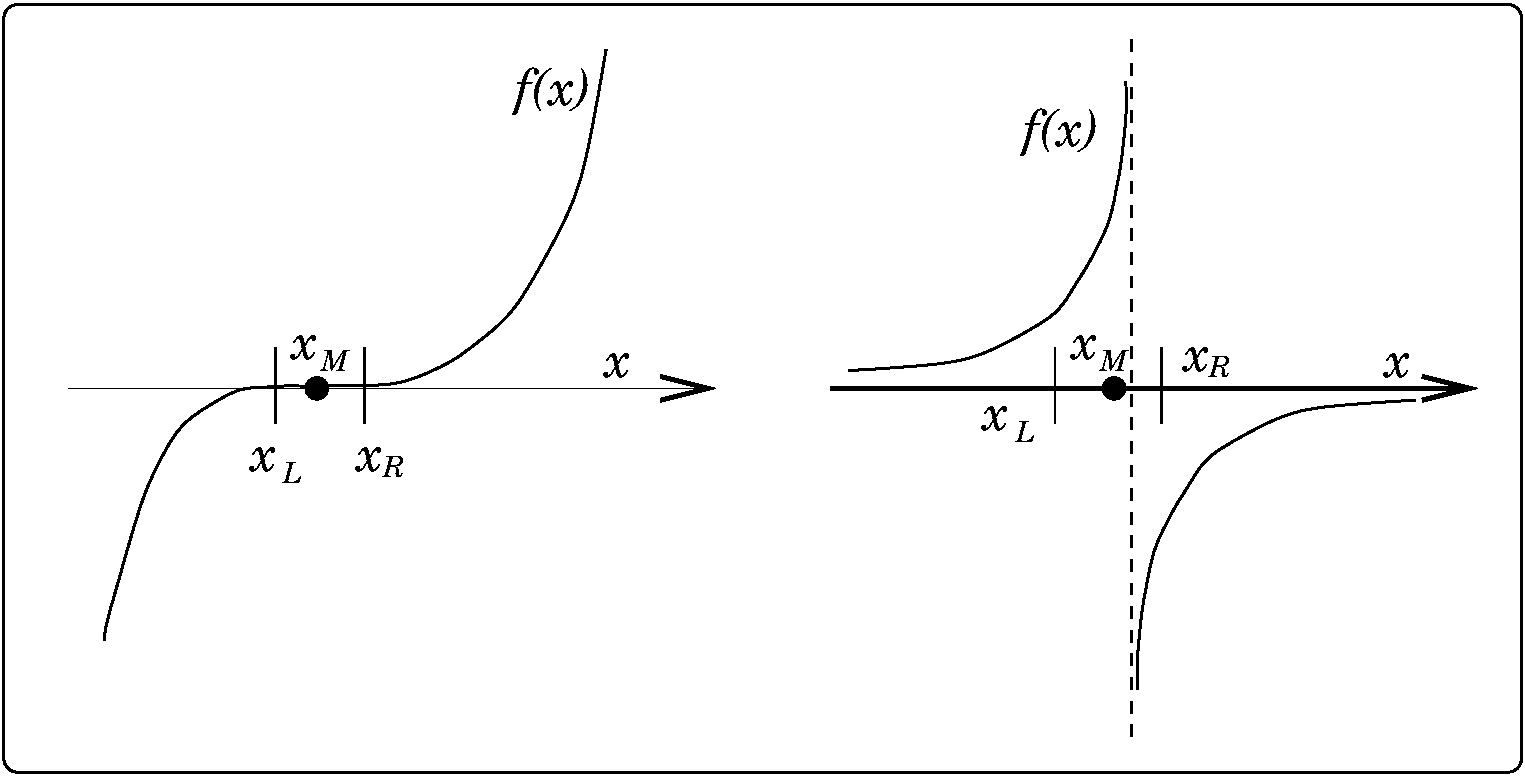
\includegraphics[width=120mm]{figures/bisec_stop}}
  \caption{\label{bisec_stop} \it In the left hand case the criterion
    $\abs{x_n^{(R)}-x_n^{(L)}} < \delta$ fails, in the right hand case the
    criterion $\abs{f(x_n^{(M)})} < \varepsilon$ fails.}
\end{figure}

\noindent
\textbf{Remark 1} - The error in the location of the root at the
$n$-th step is smaller than $(x_0^{(R)}-x_0^{(L)})/2^n$.

\noindent
\textbf{Remark 2} - This method is easy to code and it
always converges.   However, it is rather slow.

\section{Contraction mappings}

\subsection{Introduction}

Many of the methods that we will discuss for solving nonlinear
equations like
%
\begin{equation}
  f(x)=0 \label{nonlin}
\end{equation}
%
are \textit{iterative} and can be written in the form
%
\begin{equation}
  x_{n+1} = g(x_n), \label{picard}
\end{equation}
%
for some suitable function $g(x)$ and initial approximation $x_0$.
The aim of the method is to find a suitable function $g(x)$ such that
the sequence has a limit and that the limit is a root of $f(x)$:
%
\begin{equation*}
  \lim_{n \to \infty} x_n = s \quad \text{and} \quad f(s)=0.
\end{equation*}
%
Note that if the limit exists then it is also a fixed point of the map
$g(x)$:
%
\begin{equation*}
  s = \lim_{n \to \infty} x_{n+1} =
  \lim_{n \to \infty} g(x_n) =
  g \left ( \lim_{n \to \infty} x_n \right ) = g(s) .
\end{equation*}
%
For example, in the case of the nonlinear problem $f(x) = 0$ we can
define the function $g(x)$ to be
%
\begin{equation*}
  g(x) = x - f(x)
\end{equation*}
%
and use the mapping~(\ref{picard}) to attempt finding the roots of
$f(x)$.  Methods of this kind are called \textit{functional iterations
  methods} or \textit{fixed point methods}.

Graphically, the solutions of~(\ref{nonlin}) or the fixed points
of~(\ref{picard}) are the intersections between the graph of $g(x)$
and the line $y=x$ (see Figure~\ref{fig:picard}).  The iteration of
the map~(\ref{picard}) can be represented on the same graph (see
Figure~\ref{fig:picard}): in the case of the solid line path the
method is converging to the fixed point, while for the dashed line
path the method is diverging.

\begin{figure}
  \centerline{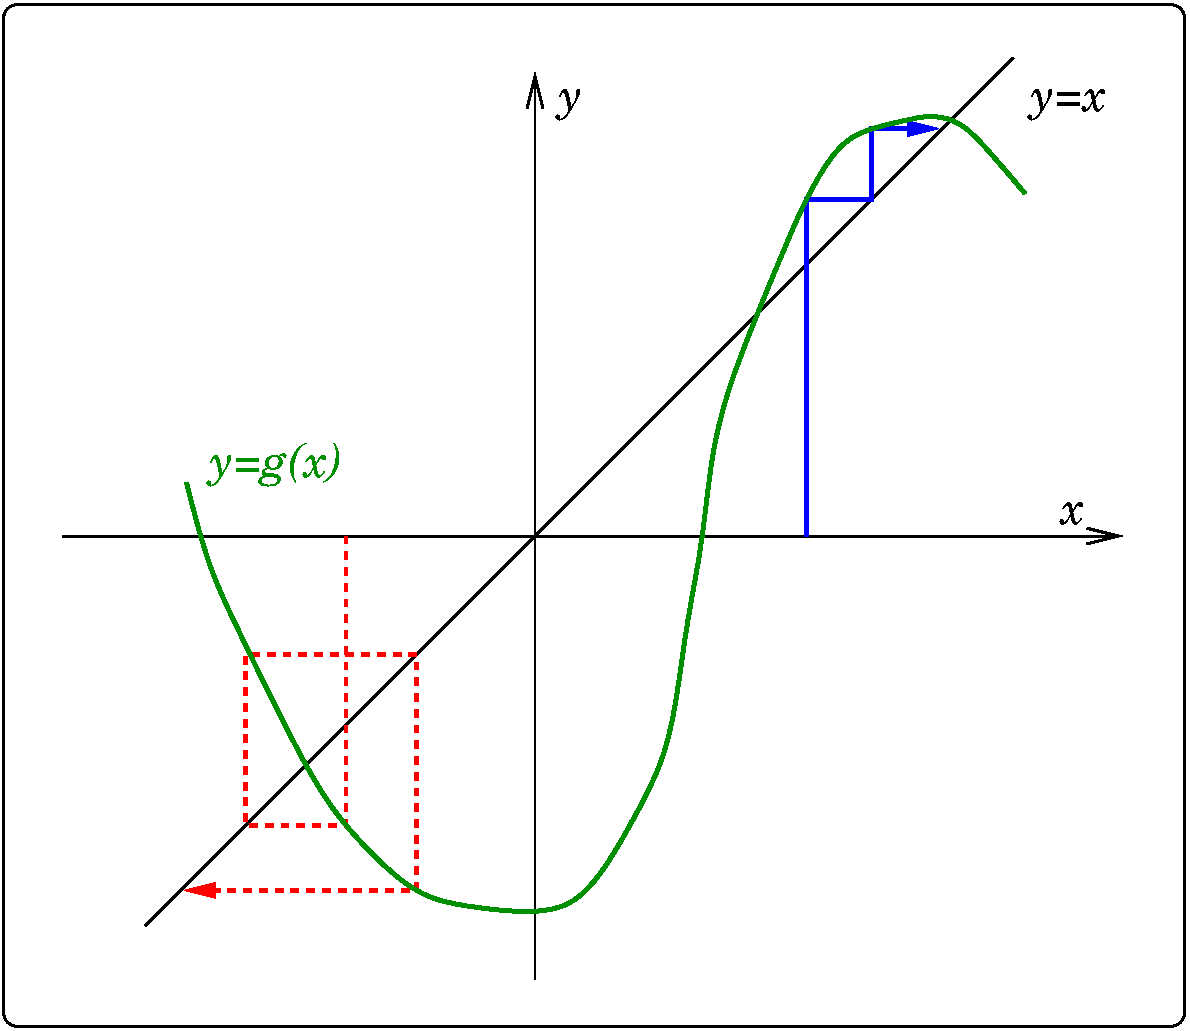
\includegraphics[width=100mm]{figures/picard}}
  \caption{\label{fig:picard} \it Graphical representation of the
    functional iteration.  The straight line paths are the graphical
    representation of the mapping~(\ref{picard}).}
\end{figure}

There are some general theorems that state under what condition the
mapping~(\ref{picard}) converges.   Before studying them, however, it
is worthwhile to make some general remarks.

\begin{itemize}
%
\item Usually iterative methods are valid for real and complex roots.
  However, in the latter case complex arithmetic must be incorporated
  into the appropriate computer codes and the initial estimate of the
  root must usually be complex.
%
\item The iterative methods require at least one initial estimate or
  guess at the location of the root being sought. If this initial
  estimate is ``sufficiently close'' to a root, then, in general, the
  procedure will converge.  The problem of how to obtain such a
  ``good'' estimate is unsolved in general.
%
\item As a general empirical rule, the schemes which converge more
  rapidly (i.e.\ higher order methods) require closer estimates.  In
  practice, these higher order schemes may require the use of more
  significant digits in order that they converge as theoretically
  predicted.  Thus, it is frequently a good idea to use a simple
  method to start with and then, when fairly close to the root, to use
  some higher order method for just a few iterations.
%
\end{itemize}

\subsection{Geometrical interpretation of fixed point schemes}

Before discussing formally what properties a map must have in order
for the iteration scheme~(\ref{picard}) to converge, we can obtain an
approximate idea by considering the four maps in
Figure~\ref{fig:contract_examples}.    From the top two maps it is
clear that in order to have a fixed point we must require $g(x)$ to be
continuous (top left) and, moreover, that the range is contained in
the domain (top right).    These requirements are not enough to have a
unique fixed point as it is shown in the bottom left corner: if the
slope of the map is too high there may be two or more fixed points.
It is only if the slope is smaller than unity that there can be only
one fixed point (bottom right corner).   Note than we do not require
that map to be differentiable: it can have as many corners as it wish.
The case of the two bottom maps is illustrated pictorially in
Figure~\ref{fig:contraction}: at each iteration the image of
the starting set $I$ gets smaller and smaller until it reduces to a
point (see Figure~\ref{fig:contraction}).

\begin{figure}
  \centerline{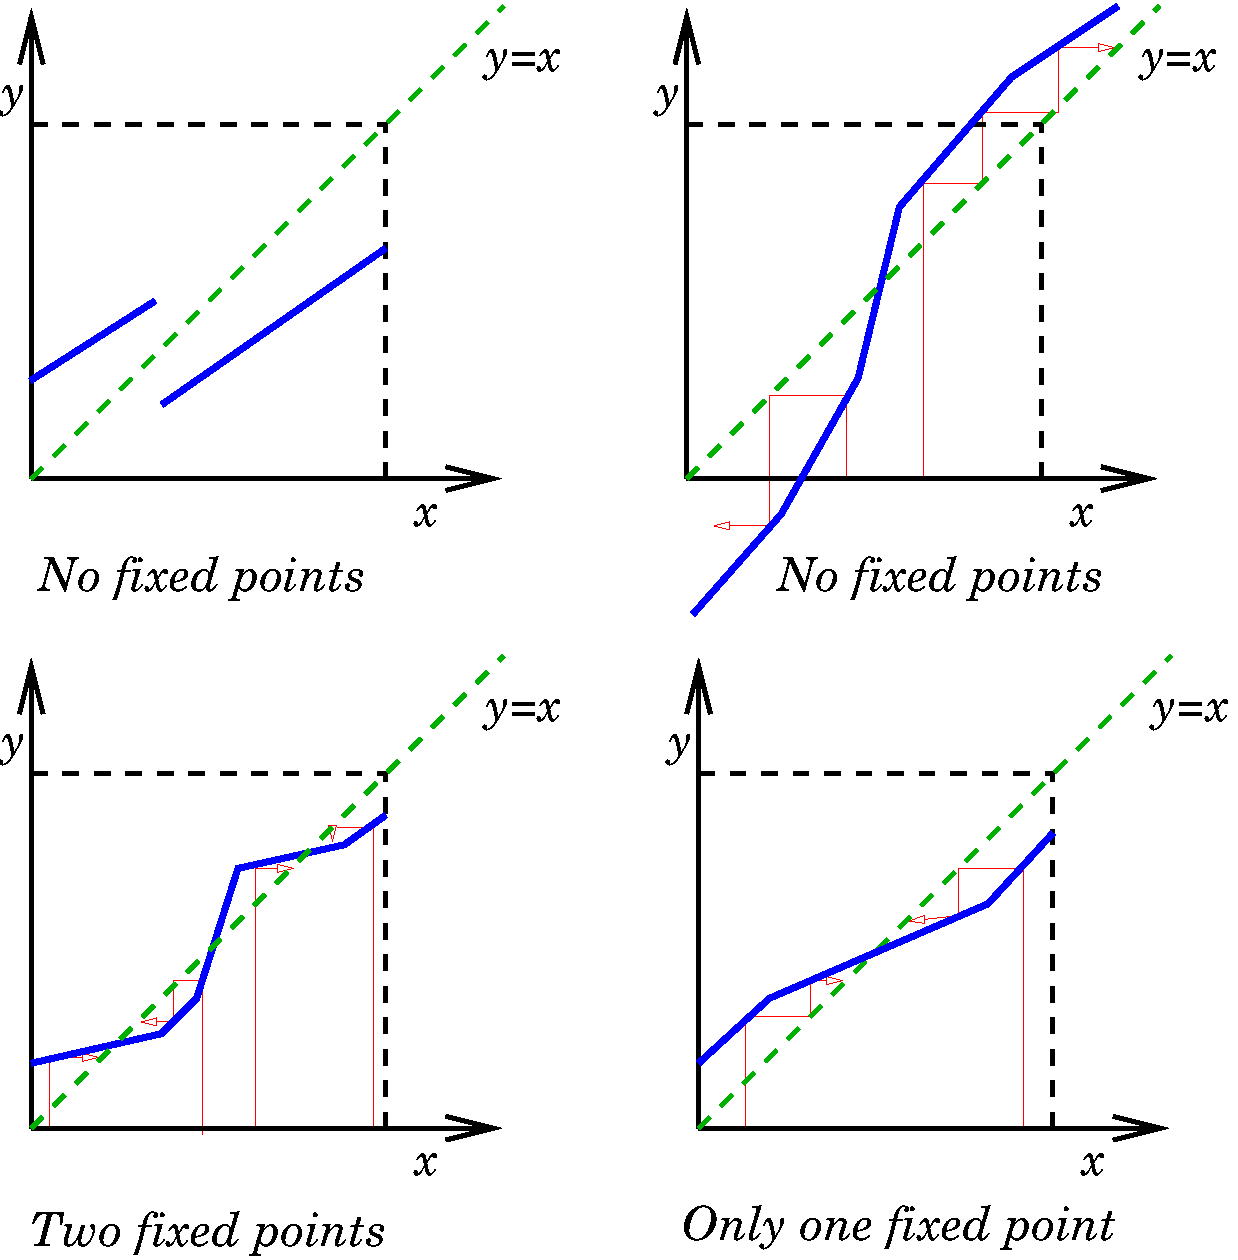
\includegraphics[width=90mm]{figures/contract_examples}}
  \caption{\label{fig:contract_examples} \it Examples of maps and
    their convergence properties.}
\end{figure}

\subsection{Definitions}

We must now phrase these intuitive results in more formal terms.   We
start by defining a contracting map.

\noindent
\textbf{Definition} - A continuous map $g(x)$ from an interval
$I=[a,b] \subseteq \bR$ into $\bR$ is \textit{contracting} if
%
\begin{enumerate}
  %
\item the image of $I$ is contained in $I$:
  %
  \begin{equation*}
    g(I) \subseteq I \quad \Leftrightarrow \quad
    g(x) \in I \, \forall x \in I .
  \end{equation*}
  %
\item the function $g(x)$ is Lipschitz continuous in $I$ with
  Lipschitz constant $L < 1$:
  %
  \begin{equation*}
    \abs{ g(x) - g(y) } \le L \abs{ x - y } \quad \forall x,y \in I .
  \end{equation*}
  %
  In other words, the distance between the images is smaller than the
  distance between the two starting points.
  %
\end{enumerate}

\noindent
\textbf{Remark 1} - A function that is Lipschitz continuous is
``more'' than continuous, but ``less'' than differentiable.  For
example, the function $f_1(x)=\sqrt{x}$ is continuous in the interval
$[0,1]$, but it is not Lipschitz.  On the other hand, the function
$f_2(x)=\abs{x}$ is Lipschitz in the interval $[-1,1]$, but it is not
differentiable at $x=0$.

\noindent
\textbf{Remark 2} - If the function $g(x)$ is differentiable and
Lipschitz continuous with constant $L$ then
%
\begin{equation*}
   \abs{\dv{g}{x}}  \le L.
\end{equation*}

\subsection{Convergence theorems}

A map that is contracting is also called a \textit{contraction
mapping}.  From the definition and Figures~\ref{fig:contract_examples}
and~\ref{fig:contraction} we can intuitively understand that if
the map $g(x)$ in~(\ref{picard}) is contracting, then we are
guaranteed convergence.  All this is expressed more
formally (and more clearly) in the following sets of theorems.

\begin{figure}
  \centerline{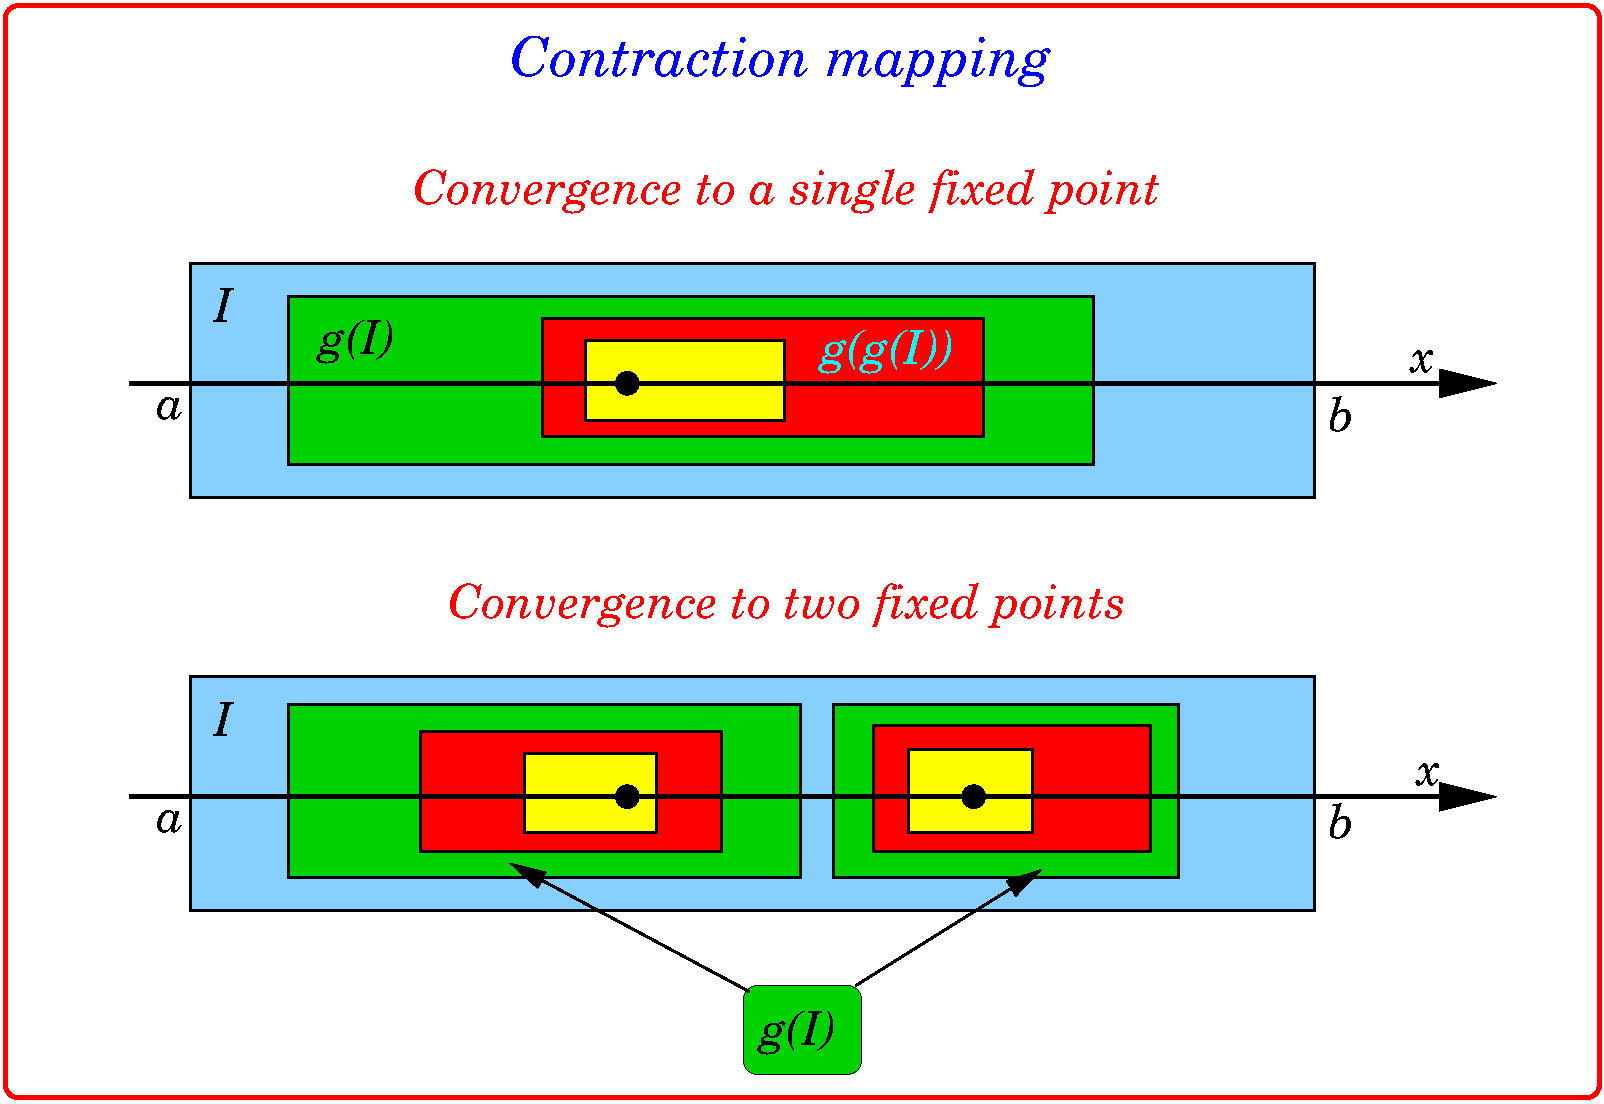
\includegraphics[width=90mm]{figures/contraction_col}}
  \caption{\label{fig:contraction} \it Graphical representation of the
    contraction mapping principle.  At each iteration the image of the
    interval gets smaller and the iterations of the contraction map
    converge towards its fixed point(s).}
\end{figure}

First of all, we prove that if the image of  the interval is contained
in the interval (without any requirement of Lipschitz continuity) then
there is at least one fixed point (but there may be many).

\smallskip

\begin{theorem}
\label{contract1}
If the function $g(x)$ is continuous in $I=[a,b]$ and $g(I) \subseteq
I$, then $g(x)$ has at least one fixed point in $I$.
\end{theorem}

\noindent
\textbf{Proof} - Since $g(I) \subseteq I$ we must have
%
\begin{equation*}
   a \le g(a) \le b \quad \text{and} \quad a \le g(b) \le b .
\end{equation*}
%
If either $g(a)=a$ or $g(b)=b$ then there is one fixed point and the
theorem is proved.   Otherwise, the following inequalities must hold:
%
\begin{equation*}
  g(a) - a \ge 0 \quad \text{and} \quad g(b) - b \le 0 .
\end{equation*}
%
Define the function $F(x) = g(x) - x$.   $F(x)$ is continuous and
$F(a) \ge 0$, while $F(b) \le 0$.   Therefore, by the intermediate
value theorem there exists a point $c \in [a,b]$ such that
%
\begin{equation*}
  F(c)=0 \implies c = g(c) .
\end{equation*}

\hfill \rule{3mm}{3mm}

\smallskip

\noindent
\textbf{Exercise} - Give a graphical representation of this theorem.
In particular show that the contraction map that would produce a graph
similar to the bottom part of Figure~\ref{fig:contraction} must have a
jump discontinuity in $[a,b]$.

\smallskip

Theorem~\ref{contract1} provides us with an important result, but not
with enough.  Ideally we would like the zero to be unique.  In order
for this to be true, we must have more stringent requirements on
$g(x)$: it must not vary too rapidly.  This is assured if $g(x)$ is
Lipschitz continuous with a sufficiently small Lipschitz constant.

\begin{theorem}[Contraction mapping theorem]
\label{contract2}
If $g(x)$ is a contraction mapping in an interval
$I=[a,b]$ then there exists one and only one fixed point of the map in
$[a,b]$.
\end{theorem}

We will prove a slightly less strong version of this theorem: we
require that the map $g(x)$ is differentiable in $I$ and that $\abs{g'(x)}
\le L < 1$.   Such a function is Lipschitz continuous of Lipschitz
constant $L$: therefore it is a contraction mapping.

\begin{theorem}
\label{contract3}
If $g(x)$ is a differentiable contraction mapping
in an interval $I=[a,b]$, i.e.
%
\begin{equation*}
  \abs{g'(x)} \le L < 1, \qquad \forall x \in [a,b] ,
\end{equation*}
%
then there exists one and only one fixed point of the map in $[a,b]$.
\end{theorem}

\noindent
\textbf{Proof} - The existence of the derivative implies that the
function $g(x)$ is continuous.  Since, by hypothesis $g(I) \subseteq
I$, then by Theorem~\ref{contract1} there is at least one fixed point,
$s_1$.  Suppose that there is another one $s_2 : s_2 = g(s_2)$ and
$s_1 \ne s_2$.  We can use the mean value
theorem\footnote{\textbf{Mean value theorem} - For any differentiable
$F(x)$ in $I \subseteq \bR$ and any $c, d \in I$ there exists a point
$\xi \in [c,d]$ such that
%
\begin{equation*}
  F'(\xi) = \frac{F(d)-F(c)}{d-c} .
\end{equation*}
}
to prove that this is impossible:
%
\begin{equation*}
  \abs{s_2 - s_1} = \abs{g(s_2) - g(s_1)} =
  \abs{g'(\xi) (s_2 - s_1)}  \le L \abs{s_2 - s_1} < \abs{|s_2 - s_1} .
\end{equation*}
%
This inequality cannot be true and therefore there can be no other
fixed point. (The proof assuming Lipschitz continuity only is
essentially identical.) \hfill \rule{3mm}{3mm}

\smallskip

The consequence of this theorem is that the algorithm represented by
the mapping~(\ref{picard}) is guaranteed to have a root in an interval
$[a,b]$ if the map is a contraction mapping in this interval.  The
following theorem tells us how to find it.

\smallskip

\begin{theorem}
\label{contract4}
Let $I=[a,b]$ and suppose that $g(x)$ is a contraction mapping in $I$.
Then for arbitrary $x_0 \in I$, the sequence $x_n = g(x_{n-1})$,
$n=1,2,\ldots$ converges to the unique fixed point, $s$, of the map.
Moreover, if the error $e_n$ at the $n$-th stage is defined by $e_n =
x_n - s$ then
%
\begin{equation*}
  \abs{e_n} \le \frac{L^n}{1-L} \abs{ x_1 - x_0 } .
\end{equation*}
\end{theorem}

\noindent
\textbf{Proof} - To prove the convergence to the fixed point, whatever
the arbitrary guess $x_0 \in I$, we use the Lipschitz property of the
map and the fact that $s=g(s$) to bound $\abs{e_n}$ from above
with a bound that tends to zero as $n$ tends to infinity.  As a first step
we have:
%
\begin{align}
  \abs{e_n} & = \abs{ x_n - s} \\
  & = \abs{ g(x_{n-1}) - g(s) } \\
  & \le L \abs{ x_{n-1} - s } \\
  & = L \abs{ e_{n-1} } .
\end{align}
%
By applying this inequality over and over again we obtain
%
\begin{align}
  \abs{ e_n } & \le L \abs{ e_{n-1} } \\
  & \le L^2 \abs{ e_{n-2} } \\
  & \le \ldots \\
  & \le L^n \abs{ e_0 } \label{ineq_conv}
\end{align}
%
By the definition of contraction mapping $L < 1$ and therefore
%
\begin{equation*}
  \lim_{n \to \infty} L^n = 0 \implies \lim_{n \to \infty} x_n = s .
\end{equation*}
%
Equation~(\ref{ineq_conv}) provides a bound on the error of the $n$-th
estimate in terms of the initial error.   Unfortunately this quantity
is not know, because we do not know the root $s$ of the equation.   We
therefore must replace $\abs{e_0}$ in~(\ref{ineq_conv}) with an expression
that we can compute, namely $\abs{x_0 - x_1}$:
%
\begin{align}
  &&  \abs{ x_0 - s } & = \abs{ x_0 - x_1 + x_1 - s } \\
  &&  & \le \abs{ x_0 - x_1 } + \abs{ x_1  - s} \\
  &&  & \le \abs{ x_0 - x_1 } + L \abs{ x_0 - s } \\
  \implies && \abs{e_0} & = \abs{ x_0 - s } \\
  && & \le \frac{\abs{ x_0 - x_1 }}{1-L}.
\end{align}
%
Using~(\ref{ineq_conv}) we obtain
%
\begin{equation}
  \abs{ e_n } \le L^n \abs{ e_0 } \le \frac{L^n}{1-L} \abs{ x_0 - x_1 } .
  \label{err_boundL}
\end{equation}
\hfill \rule{3mm}{3mm}

These four theorems are represented graphically in
Figure~\ref{fig:contract}.  Since the slope of the function $g(x)$ is
smaller than unity successive iterations of the map get closer and
closer to its fixed point.

\begin{figure}
  \centerline{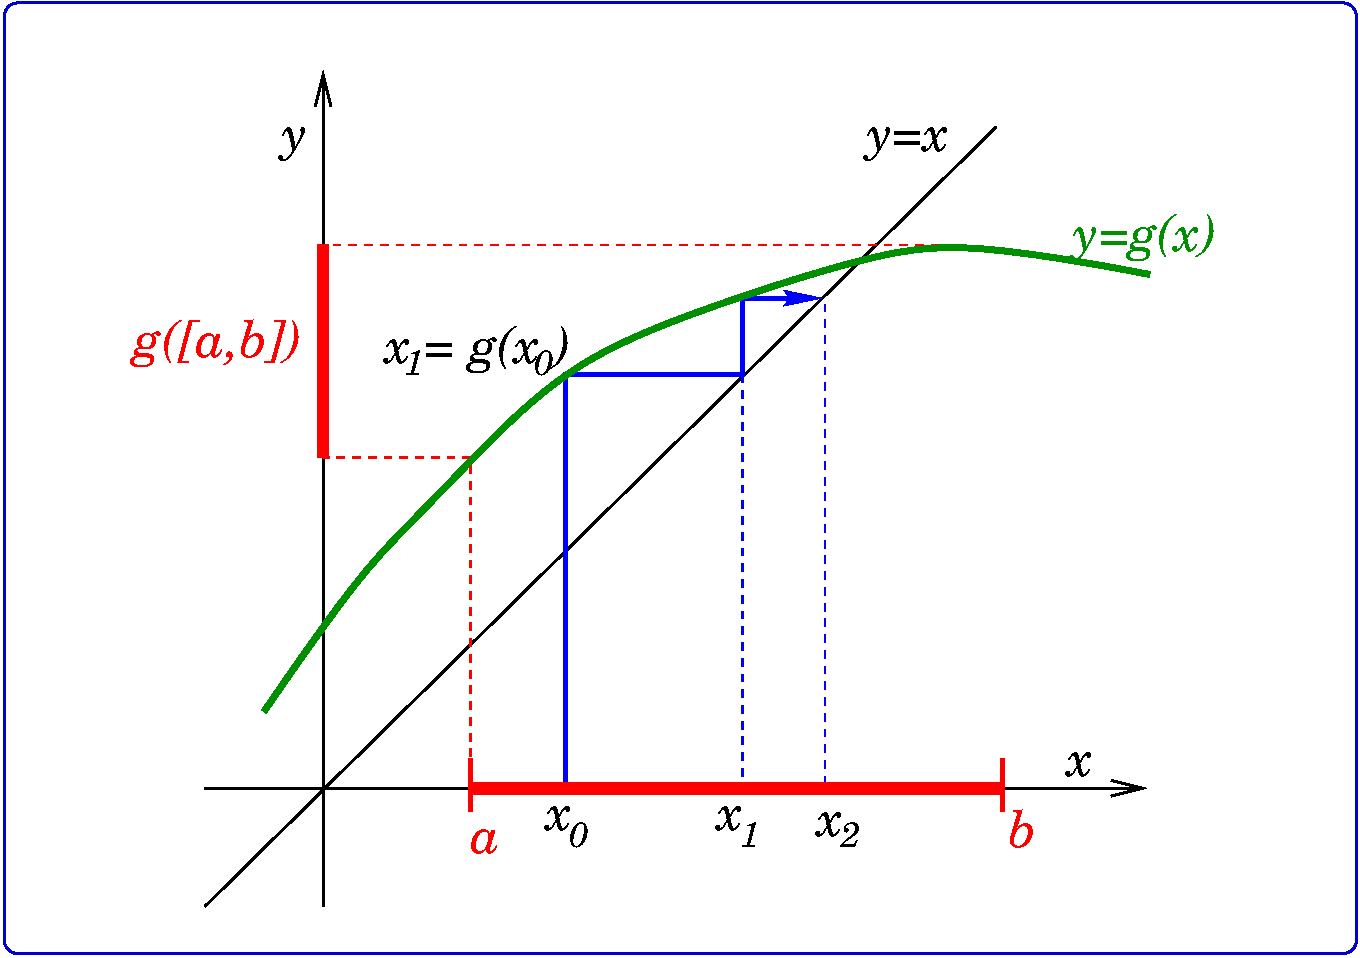
\includegraphics[width=80mm]{figures/contract}}
  \caption{\label{fig:contract} \it Graphical representation of the
    contracting mapping theorems.  The map $g(x)$ is a contraction
    mapping in $[a,b]$: the image of the interval is smaller than the
    original interval.  Each iteration of a starting guess $x_0$ gets
    closer and closer to the fixed point.}
\end{figure}

\subsection{Speed of convergence}

The bound~(\ref{err_boundL}) on the error provided by
Theorem~\ref{contract4} depends, through the Lipschitz constant $L$,
on the interval chosen to estimate the map.  Moreover, it is
reasonable to assume that the rate of convergence of the map, i.e.\ the
rate of decrease of the error $e_n$ depends only on the properties of
the map in a neighbourhood of the root.  We can show that this is
indeed the case if the map is differentiable, so that it is possible
to expand it in a Taylor polynomial: call $g(x)$ a suitably
differentiable contraction mapping in $I=[a,b]$, $s$ its fixed point,
$x_0 \in I$ the starting point of the iteration and $e_n = x_n - s$
the error at the $n$-th iteration.  Using the definition of the map
and Taylor's expansion we can write:
%
\begin{align*}
  e_{n+1} & = x_{n+1} - s \\
          & = g(x_n) - g(s) \\
          & = g'(s)(x_n-s) + \frac{g''(s)}{2!}(x_n-s)^2 + \ldots +
          \frac{g^{(k)}(s)}{k!}(x_n-s)^k + R_{n,k} \\
          & = g'(s) e_n + \frac{g''(s)}{2!} e_n^2 + \ldots +
          \frac{g^{(k)}(s)}{k!} e_n^k + R_{n,k} ,
\end{align*}
%
where $R_{n,k}$ is the remainder of the expansion:
%
\begin{equation*}
  R_{n,k} = \frac{g^{(k)}(\xi)}{k!}(x_n-s)^{k+1}, \quad
  \xi \in [x_n,s].
\end{equation*}
%
Assuming that $g'(s) \ne 0$ then
%
\begin{equation*}
  e_{n+1} \sim g'(s) e_n,
\end{equation*}
%
i.e.\ the error decreases at a constant rate at each iteration: such a
method is called \textit{linear} or \textit{first order}.  If,
instead, $g'(s)=0$, but $g''(s) \ne 0$ then
%
\begin{equation*}
  e_{n+1} \sim g''(s) e_n^2,
\end{equation*}
%
i.e.\ the error at each iteration is proportional to the square of the
previous error: such a method is called a \textit{quadratic} or
\textit{second order} method.  The more derivatives of $g(s)$ vanish
the higher the order of the method and the faster the convergence.
However, it may well be that the method will converge only if the
starting point is very close to the root.

\subsection{Error propagation}

The final question that we must answer before discussing practical
implementations of the theory we have just studied is ``Are these
theorems numerically stable?''  In other words, what is the effect of
the numerical error on the convergence properties of a contraction
map?  In actual computations it may not be possible, or practical, to
evaluate the function $g(x)$ exactly (i.e.\ only a finite number of
decimals may be retained after rounding or $g(x)$ may be given as the
numerical solution of a differential equation, etc.).  For any value
of $x$ we may then represent our approximation to $g(x)$ by $G(x) =
g(x) + \delta(x)$ where $\delta(x)$ is the error committed in
evaluating $g(x)$.  Frequently we may know a bound for $\delta(x)$,
i.e.\ $\delta(x) < \delta$.  Thus the actual iteration scheme which is
used may be represented as
%
\begin{equation}
  X_{n+1} \equiv G(X_n) = g(X_n) + \delta_n, \quad
  n = 0,1,2, \ldots, \label{Xn}
\end{equation}
%
where the $X_n$ are the numbers obtained from the calculations and the
$\delta_n \equiv \delta(X_n)$ satisfy
%
\begin{equation}
  \abs{\delta_n} \le \delta, \quad n= 0,1,2, \ldots \label{deltabound}
\end{equation}
%
We cannot expect the computed iterates $X_n$ of~(\ref{Xn}) to
converge.   However, under proper conditions, it should be possible to
approximate a root to an accuracy determined essentially by the
accuracy of the computations, $\delta$.

\begin{figure}
  \centerline{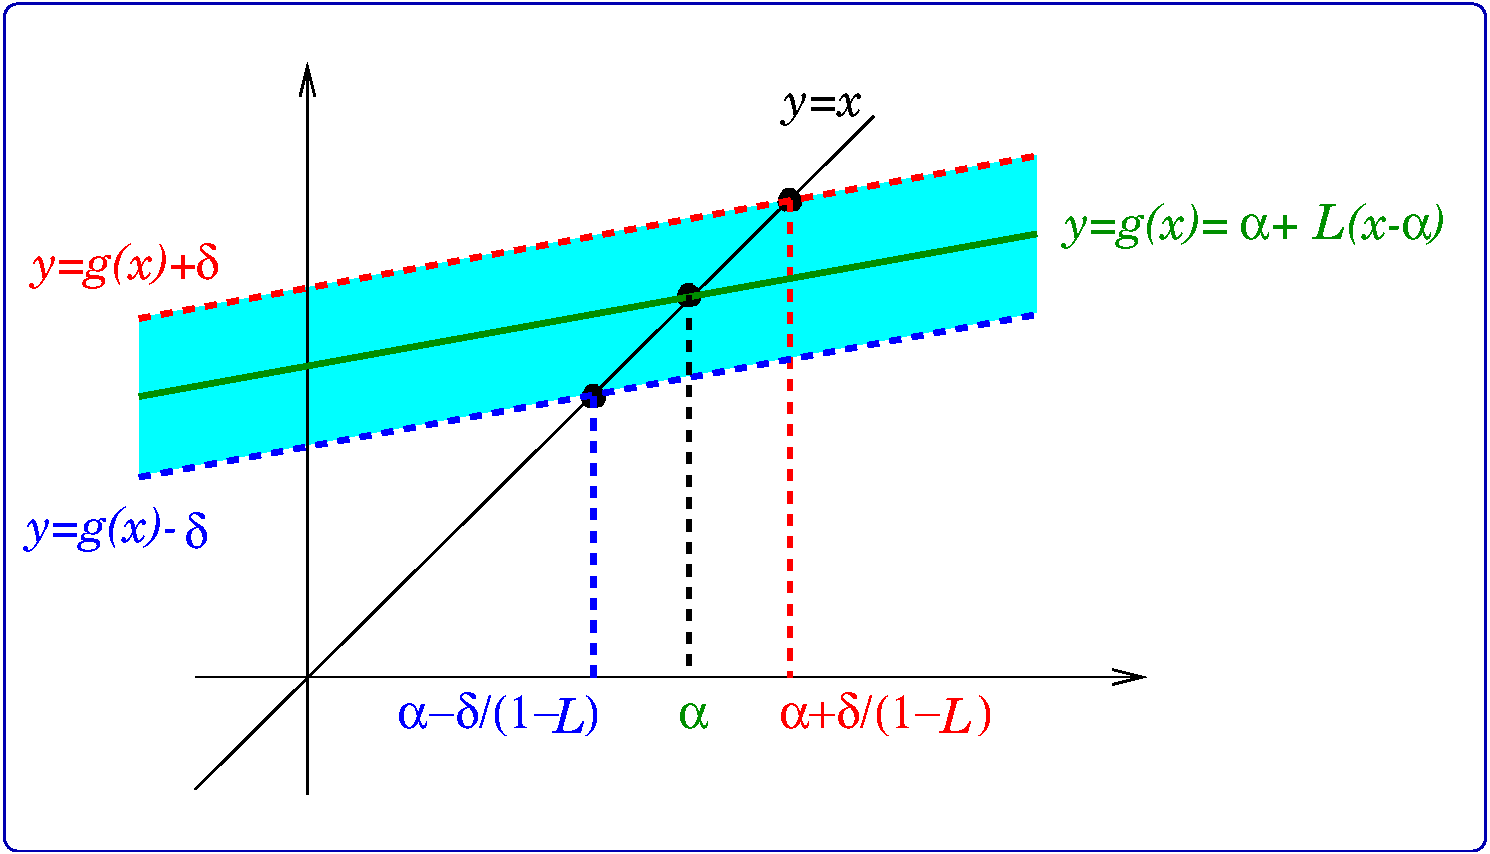
\includegraphics[width=120mm]{figures/contract_error}}
  \caption{\label{fig:contract_error} \it The width of the numerical
    error band around the fixed point of the iteration map.}
\end{figure}

For example, from Figure~\ref{fig:contract_error} we can see that for
the special case of $g(x) = \alpha + L (x-\alpha)$, the uncertainty in
the root $\alpha$ is bounded by $\pm \delta/(1 - L)$.  We note that if
the slope $L$ is close to unity the problem is not ``properly posed''.
The following theorem states quite generally that when the functional
iteration scheme is convergent, the presence of errors in computing
$g(x)$, of magnitudes bounded by $\delta$, causes the scheme to
estimate the root $\alpha$ with an uncertainty bounded by $\pm
\delta/(1-L)$, where $L$ is the Lipschitz constant of the contraction
mapping.  The phrasing of this theorem is slightly different from the
previous ones because the numerical error $\delta$ forces us to define
quite strictly the interval we want to work in: we know that $g(I)
\subseteq I$, but it is not generally true that $G(I) \subseteq I$.

\begin{theorem}
\label{contract5}
Let $g(x)$ be a contraction mapping with fixed point $s$ and let $L$
be its Lipschitz constant in the interval $I(s,r_0) \equiv
[s-r_0,s+r_0]$.  Let $\delta$ be the bound on the numerical errors of
the iterates of the numerical map~(\ref{Xn}) as defined
in~(\ref{deltabound}).  Finally, assume that the starting point of the
iteration of~(\ref{Xn}) is a point $X_0$ in the smaller interval
%
\begin{equation}
  X_0 \in I(s,R_0) \equiv [s - R_0, s + R_0] ,  \label{X0}
\end{equation}
%
where
%
\begin{equation*}
  0 < R_0 \le r_0 - \frac{\delta}{1-L} .
\end{equation*}
%
Then the iterates $X_n$ of~(\ref{Xn}) with the errors bounded
by~(\ref{deltabound}), lie in the interval $I(s,r_0)$,
and
%
\begin{equation}
  \abs{ s - X_n } \le
  \frac{\delta}{1 - L} +
  L^n \left ( R_0 - \frac{\delta}{1-L} \right ), \label{bound_err}
\end{equation}
%
where $L^n \to 0$ as $n \to \infty$.
\end{theorem}

\noindent
\textbf{Proof} - The proof of this theorem involves showing that the
numerical error does not push the iteration outside the interval
$I(s,r_0)$ where it is defined.  In the process of doing so we also
derive the bound~(\ref{bound_err}) on the error of the numerical
estimate.  The proof that the iterations are always in the interval
$I(s,r_0)$ is by induction.

The point $X_0$ is, by hypothesis, inside the interval $I(s,R_0)
\subseteq I(s,r_0)$.  We now suppose that the iterations $X_0, X_1,
\ldots, X_{n-1}$ are in $I(s,r_0)$ and proceed to show that also $X_n
\in I(s,r_0)$.  By~(\ref{Xn}) and~(\ref{deltabound}) we have
%
\begin{equation*}
  \abs{ s - X_n } \le
    \abs{ [g(s) - g(X_{n-1}) ] - \delta_{n-1}  } \le
  \abs{ [g(s) - g(X_{n-1}) ]  } + \delta .
\end{equation*}
%
Since $g(x)$ is a contraction mapping of Lipschitz constant $L$  we
can write
%
\begin{align*}
  \abs{ s - X_n } & \le L \abs{ s - X_{n-1} } + \delta \\
  & \le L^2 \abs{ s - X_{n-2} } + L \delta + \delta \\
  & \le L^n \abs{ s - X_0} + ( L^{n-1} + \ldots 1 ) \delta \\
  & =  L^n \abs{ s - X_0} + \frac{1-L^n}{1-L} \delta .
\end{align*}
%
Hypothesis~(\ref{X0}) implies that $\abs{s - X_0} \le R_0$ so that
%
\begin{align}
  \abs{ s - X_n } & \le L^n R_0 + \frac{1-L^n}{1-L} \delta  \label{be1} \\
  & = L^n R_0 + \frac{\delta}{1-L} - L^n \frac{\delta}{1-L} \nonumber \\
  & \le R_0  + \frac{\delta}{1-L} \nonumber \\
  & \le r_0. \nonumber
\end{align}
Thus all the iterates are in the interval $I(s,r_0)$ and the iteration
process is defined.   Moreover~(\ref{be1}) can be rewritten
as~(\ref{bound_err}), thus completing the proof. \hfill \rule{3mm}{3mm}

\smallskip

\noindent
\textbf{Remark} - Theorem~\ref{contract5} shows that the method is
``as convergent as possible'', that is, the computational errors which
arise from the evaluation of $g(x)$ may cumulatively produce an error
of magnitude at most $\delta/(1-L)$.  Moreover, such errors limit the
size of the error bound \textit{independently of the number of
iterations}.  Therefore, it is pointless to iterate the map until $L^n
r_0 \ll \delta/(1-L)$.

\section{Examples of iteration procedures}

\subsection{Introduction}

We  have completed the  theoretical  introduction to the
numerical solution of nonlinear  equations.  We must now discuss  some
of the  algorithms  that apply  the   theory that  we have  developed.

\subsection{The chord method (first order)}

The chord method and Newton's methods are examples of the application
of the contraction mapping theorems.  Both these methods can be
introduced using a general and elegant framework.  As usual we suppose
that we have to solve the nonlinear equation
%
\begin{equation*}
  f(x) = 0,
\end{equation*}
%
in some interval $a \le x \le b$.  To define the different methods to
solve this problem we introduce a function $\varphi(x)$ such that
%
\begin{equation}
  0 < \varphi(x) < \infty, \quad x \in [a,b] ,
 \label{phibound}
\end{equation}
%
and we use it to construct a contraction mapping $x_{n+1} =
g(x_n)$, where
%
\begin{equation}
  g(x) = x - \varphi(x) f(x).   \label{gphi}
\end{equation}
%
The fixed points of the map $g(x)$ are the roots of the function
$f(x)$.

\smallskip

The simplest choice for $\varphi(x)$ in~(\ref{gphi}) is to take
%
\begin{align}
  && \varphi(x) & \equiv m \ne 0, \\
  \implies && g(x) & = x - m f(x) \\
  \implies && x_{n+1} & = x_n - m f(x_n)
  \label{phichord}
\end{align}
%
where $m$ is a number that we must choose appropriately in order for
$g(x)$ to be a contraction mapping in $[a,b]$.   The range of $m$
depends on the slope of $f(x)$ in the interval $[a,b]$.   From
Theorem~\ref{contract3} we know that $g(x)$ is a contraction mapping if
%
\begin{align}
  & &  \abs{ g'(x) } & < 1 &  \forall x &\in [a,b] \nonumber
  \\
  \implies &&
  \abs{ 1 - m f'(x) } & < 1 & \forall x &\in [a,b] \nonumber
  \\
  \implies && 0 < m f'(x) & < 2 & \forall x &\in [a,b] . \label{ineq_chord}
\end{align}
%
Thus $m$ must have the same sign as $f'(x)$, while if $f'(x)=0$ the
inequality cannot be satisfied.

The iterates of~(\ref{phichord}) have a geometrical realisation in
which the value $x_{n+1}$ is the $x$ intercept of the line with slope
$1/m$ through $(x_n,f(x_n))$ (see Figure~\ref{fig:chord}).   The
inequality~(\ref{ineq_chord}) implies that this slope should be
between $\infty$ (i.e.\ vertical) and $f'(x)/2$ (i.e.\ half the slope of
the tangent to the curve $y=f(x)$).   It is from this geometric
description that the name chord method is derived - the next iterate
is determined by a chord of constant slope joining a point on the
curve to the $x$-axis.

\begin{figure}
  \centerline{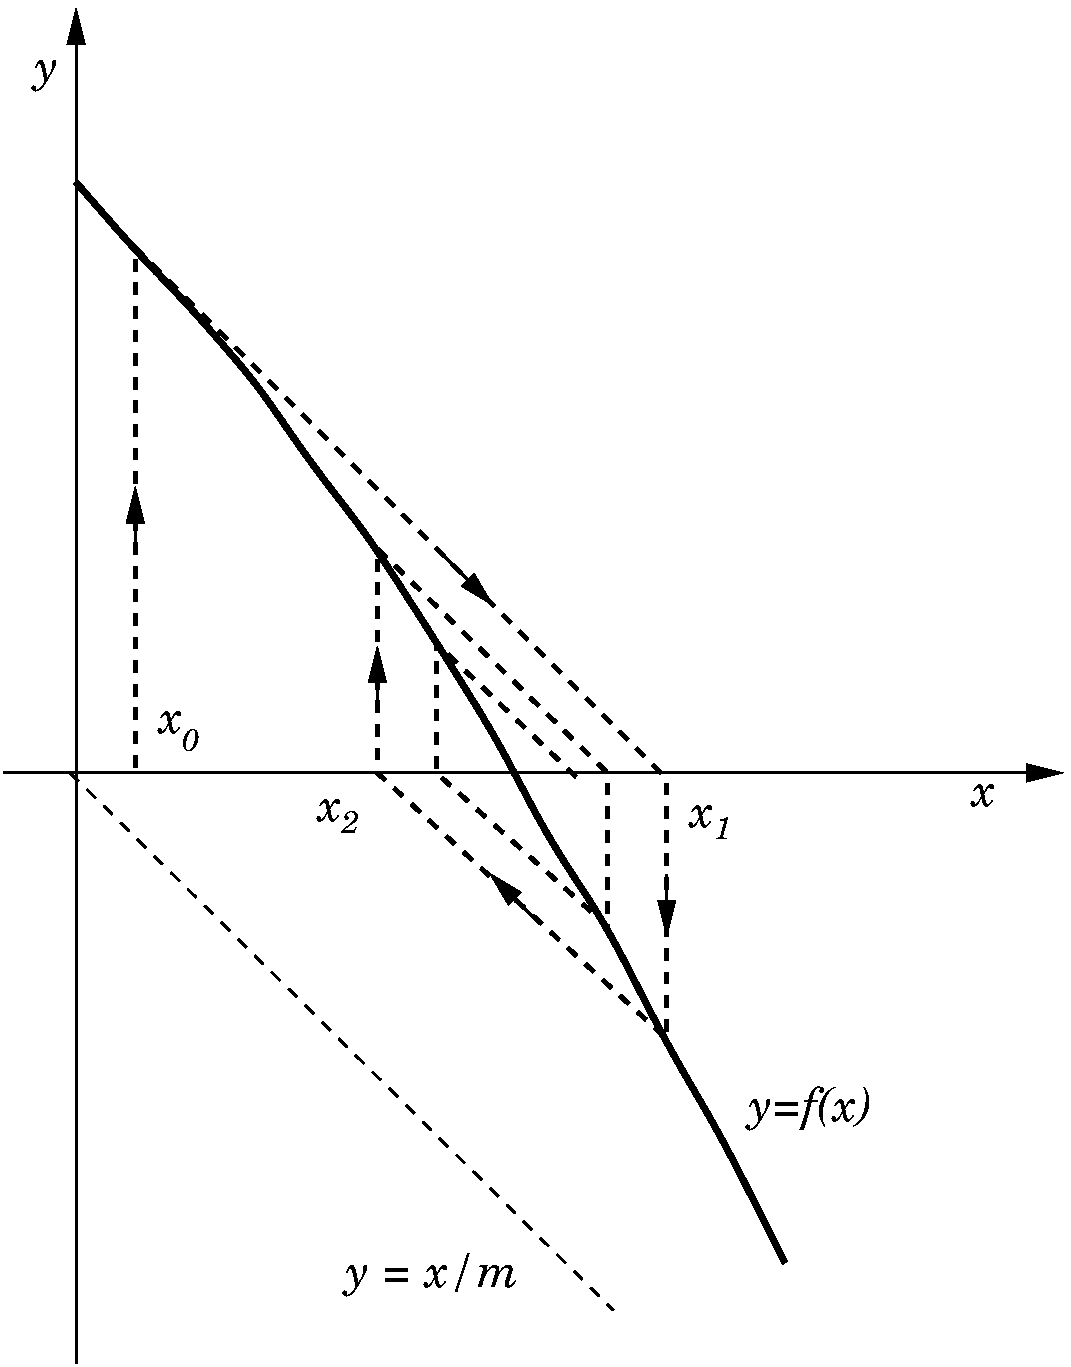
\includegraphics[width=60mm]{figures/chord}}
  \caption{\label{fig:chord} \it Geometrical representation of the
    chord method: each new iterate is determined by a chord of
    constant slope joining a point on the curve to the $x$-axis.}
\end{figure}

\medskip

\subsection{Newton's method (second order)}

The idea behind Newton's method is to chose the function $\varphi(x)$
in order that the derivative of the iteration mapping $g(x)$ is zero
at the root $x=s$.  This is ensured by the choice
%
\begin{equation}
  \varphi(x) = \frac{1}{f'(x)} \implies
  g(x) = x - \frac{f(x)}{f'(x)} , \label{gnewt}
\end{equation}
%
so that the iteration procedure is
%
\begin{equation}
  x_{n+1} = x_n - \frac{f(x_n)}{f'(x_n)} .
  \label{Newton}
\end{equation}
%
This root finding algorithm is called Newton's method.
Theorem~\ref{contract3} guarantees that the method converges in an
interval $[a,b]$ containing the root provided that $\abs{g'(x)} < 1$ in
the interval.  It is at least second order at the root $s$ of the
equation $f(x) = 0$, if $f'(s) \ne 0$ and $f''(x)$ exists, since
%
\begin{equation}
  g'(s) = \frac{f(s) f''(s)}{[f'(s)]^2} = 0 .
  \label{gpalpha}
\end{equation}
%
The geometrical interpretation of this scheme simply replaces the
chord in Figure~\ref{fig:chord} by the tangent to the line to $y=f(x)$
at $x_n,f(x_{n+1})$ (see Figure~\ref{fig:Newton}).

\begin{figure}
  \centerline{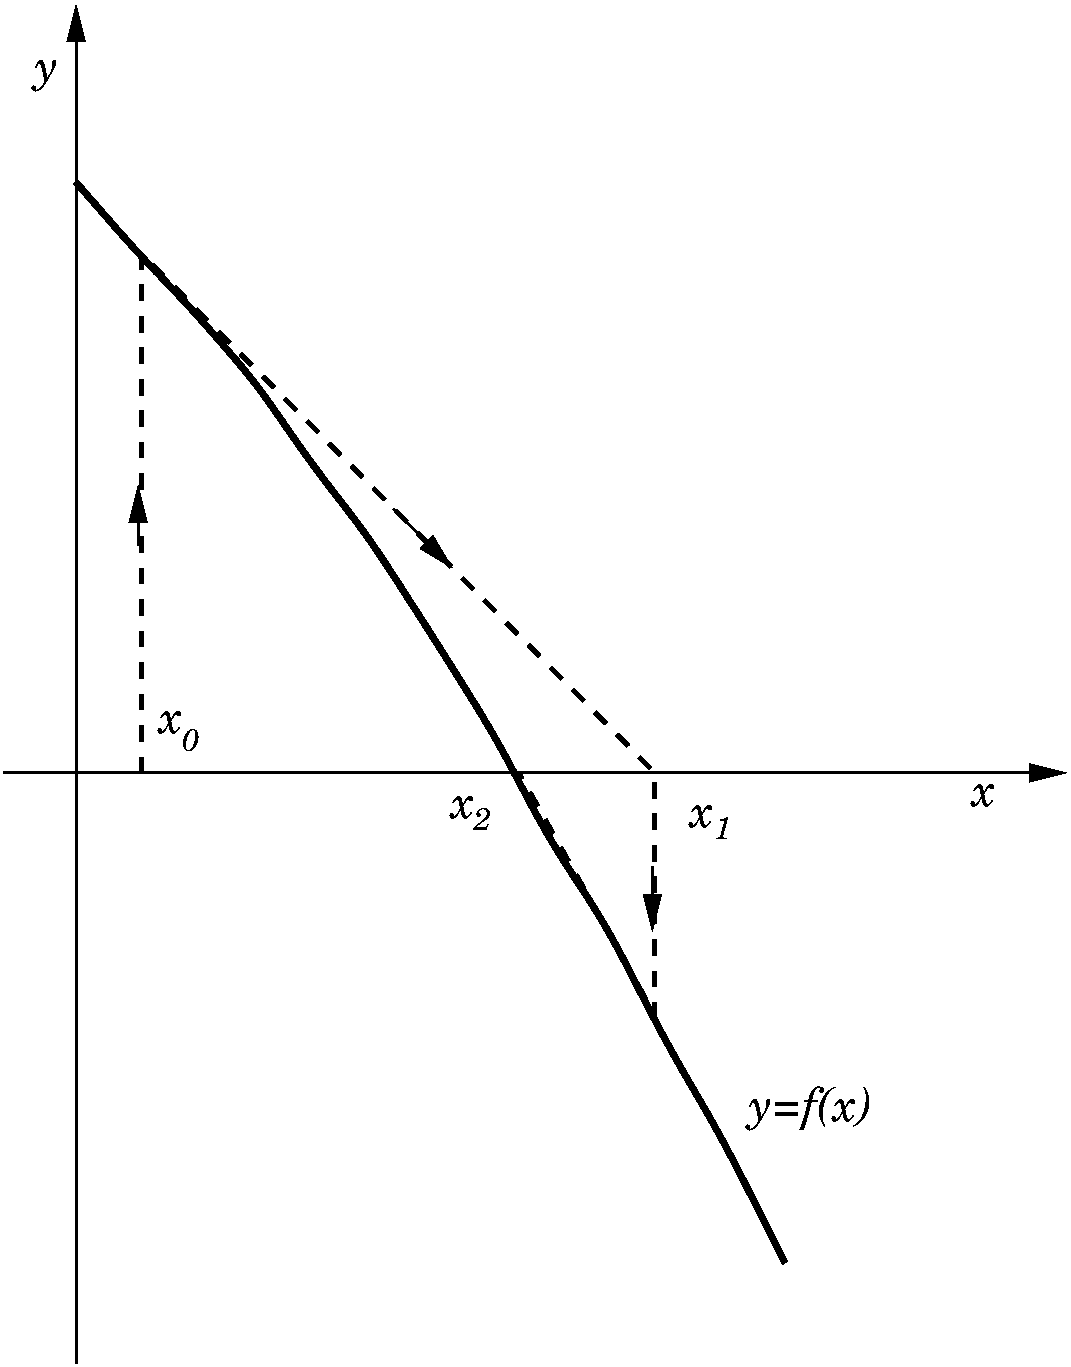
\includegraphics[width=80mm]{figures/Newton}}
  \caption{\label{fig:Newton} \it Geometrical representation of
    Newton's method: each new iterate is intersection of the tangent
    to the graph of $f(x)$ with the $x$-axis.}
\end{figure}

\noindent
\textbf{Remark 1} - It should be noted that Newton's method may be
undefined and the condition~(\ref{phibound}) violated if $f'(x)=0$ for
some $x \in [a,b]$.  In particular, if at the root $x=s$, $f'(s) = 0$,
the procedure may no longer be of second order since the hypotheses
that lead to~(\ref{gpalpha}) are not satisfied.  To examine this case
we assume that $f(x)$ has a root of multiplicity $p$ at $x=s$.  In
other words we can write,
%
\begin{equation*}
  f(x) = (x-s)^p h(x), \quad p > 1 ,
\end{equation*}
%
where the function $h(x)$ has a second derivative and $h(s) \ne 0$.
If we substitute this expression in the definition of $g(x)$
in~(\ref{gnewt}) we find that
%
\begin{equation*}
  \abs{g'(s)} = 1 - \frac{1}{p} .
\end{equation*}
%
So only in the case of a linear root, i.e.\ $p=1$ is Newton's method
second order, but it will converge as a first order method in the
general case $p \ne 1$.

\noindent
\textbf{Remark 2} - Convergence is quadratic only if we are close to
the root $s$.

\noindent
\textbf{Remark 3} - The advantage of Newton's method with respect to
the bisection (and chord) method is the faster convergence.  The main
disadvantage with respect to the bisection method is that we need to
start relatively close to the root in order to be sure that the method
will converge.

\subsection{Secant method (fractional order)}

Newton's method requires the evaluation of the derivative of the
function $f(x)$ whose root we want to find.  To do this may be very
complicated and time consuming: the secant method obviates this
problem by approximating the derivative of $f'(x)$ with the quotient
%
\begin{equation}
  f'(x_n) \simeq
  \frac{f \left (x_n \right ) - f \left ( x_{n-1} \right )}
  {x_n - x_{n-1}} .
  \label{approx_der}
\end{equation}
%
This approximation comes directly from the definition of the derivative
of $f(x)$ as the limit
%
\begin{equation*}
  f'(x) = \lim_{u \to x} \frac{f(u)-f(x)}{u-x} .
\end{equation*}
%
Substituting~(\ref{approx_der}) into the algorithm~(\ref{Newton}) for
Newton's method we obtain the secant method, namely:
%
\begin{equation}
  x_{n+1} = x_n -
  f(x_n) \frac{x_n - x_{n-1}}{f(x_n) - f (x_{n-1})} .
  \label{secant}
\end{equation}
%
The graphical interpretation of the secant method is similar to that
of Newton's method.  The tangent line to the curve is replaced by the
secant line (see Figure~\ref{fig:secant}).

\begin{figure}
  \centerline{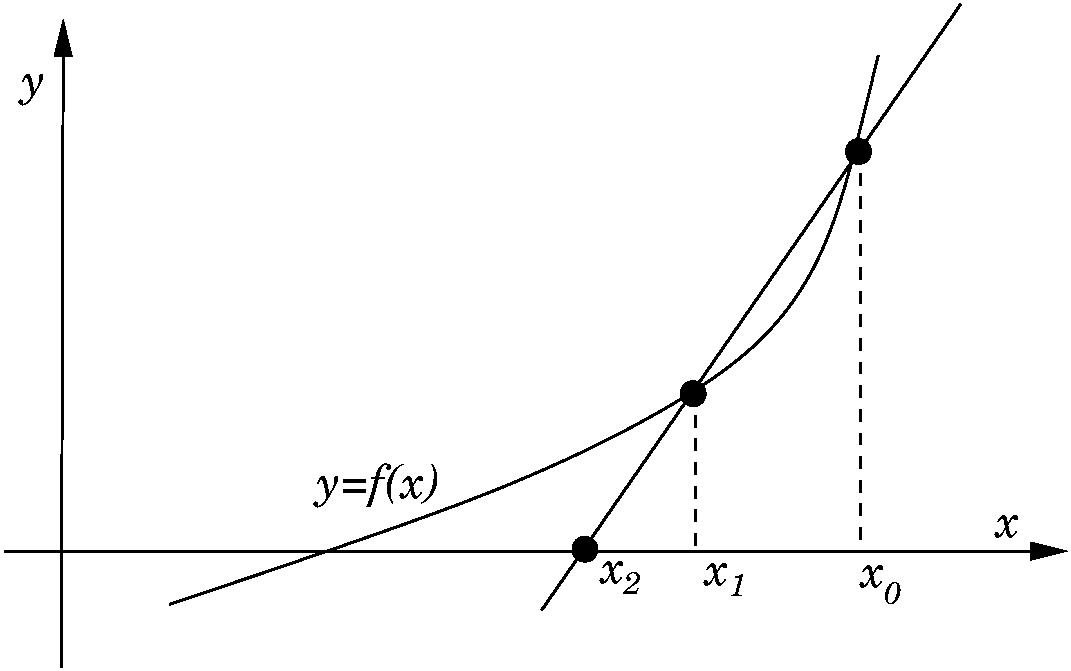
\includegraphics[width=90mm]{figures/secant}}
  \caption{\label{fig:secant} \it Geometrical representation of the
    secant method: each new iterate is intersection of the secant to
    the graph of $f(x)$ with the $x$-axis.}
\end{figure}

\noindent
\textbf{Remark 1} - This method requires two initial guesses:
$x_0$ and $x_1$.

\noindent
\textbf{Remark 2} - The convergence of the secant method cannot be
analysed using the contraction mapping theorems that we have studied
because the method cannot be put in the form $x_{n+1} = g(x_n)$: each
new iterate is a function of the previous \textbf{two}: $x_{n+1} =
g(x_n, x_{n-1})$.

\noindent
\textbf{Remark 3} - It is possible to show that the
error in the approximation decreases asymptotically as
%
\begin{equation*}
  \abs{e_{n+1}} \sim \abs{e_n}^{(1+\sqrt{5})/2} .
\end{equation*}
%
Since $(1+\sqrt{5})/2 \simeq 1.62$ the secant method is a super-linear
(i.e.\ faster than linear), but slower than quadratic convergence.
This would suggests that the secant method is slower than Newton's
method in reaching a given accuracy.  However, Newton's method
requires two function evaluations per iteration step, while the secant
method requires only one.  Therefore, when comparing the execution
speed of the two methods we should/could compare \textit{two} steps of
the secant methods with one step of Newton's method.  The rate of
decrease of the error in two steps of the secant method is $1.62^2
\simeq 2.6$ which is better than the convergence rate of Newton's
method.

\section{Systems of nonlinear equations}

\subsection{Introduction}

Finding the solutions of a systems of nonlinear equations,
%
\begin{equation*}
  \begin{cases}
    f_1(x_1, x_2, \ldots, x_n) = 0 , \\
    f_2(x_1, x_2, \ldots, x_n) = 0 , \\
    \vdots \\
    f_n(x_1, x_2, \ldots, x_n) = 0 ,
  \end{cases}
 \quad \Leftrightarrow \quad
 \bff(\bx) = 0 ,
\end{equation*}
%
is considerably more difficult that solving a single nonlinear
equation or solving a system of linear equations:

\begin{enumerate}
  %
\item The system may have \textit{no solution}, like for example
  %
  \begin{align*}
    \left\{
      \begin{aligned}
        x_1^2 + 2 x_1 x_2 + x_2^2 & = 3, \\
        x_1^3 + 3 x_1^2 x_2 + 3 x_1 x_2^2 + x_2^3 & = 4,
      \end{aligned}
    \right. &  \Longleftrightarrow \left\{
      \begin{aligned}
        (x_1 + x_2)^2 & = 3, \\
        (x_1 + x_2)^3 & = 4,
      \end{aligned}
    \right. \\
  \intertext{or have \textit{no real solutions}, like for example,}
    \left\{
      \begin{aligned}
        x_1^2 + x_2^2 & = -5, \\
        x_1^2 - 3 \, x_2^2 & = 11,
      \end{aligned}
    \right. &  \Longleftrightarrow \left\{
      \begin{aligned}
        x_1 & = \pm \tj , \\
        x_2 & = \pm 2 \tj ,
      \end{aligned}
    \right. \\
  \intertext{or have a \textit{unique solution}}
    \left\{
      \begin{aligned}
        x_1^2 + x_2^2 & = 0, \\
        \cos(x_1 x_2) & = 1,
      \end{aligned}
    \right. &  \Longleftrightarrow \left\{
      \begin{aligned}
        x_1 = 0 , \\
        x_2 = 0 ,
      \end{aligned}
    \right. \\
  \intertext{or have \textit{many solutions}}
    \left\{
      \begin{aligned}
        x_1^2 + x_2^2 & = 1, \\
        \cos[\pi(x_1^2 + x_2^2)] + x_1^2 + x_2^2 & = 0,
      \end{aligned}
    \right. &  \Longleftrightarrow
    \parbox{50mm}{all $x_1$ and $x_2$ that belong to the circle $x_1^2 +
      x_2^2 = 1$.}
  \end{align*}
  %
\item If the system is large, even the existence of a solution is
  quite unclear.
  %
\item For many real world problems the methods used to find the
  solutions can be rather ad hoc.
  %
\end{enumerate}

\subsection{Contraction mapping}

One can extend to more than one dimension the theorems on contraction
mapping that have been discussed so far.  The contraction map is now a
set of $n$ nonlinear functions in $n$ variables,
%
\begin{equation*}
  \bx_{n+1} = \bg(\bx_n) .
\end{equation*}
%
Essentially everything carries over by replacing scalars with vectors
and absolute values with norms.

We define an \textit{interval} in $\bRn$ as a set $I = \{ \bx \in \bRn
| \, a_j < x_j < b_j, \, j=1,2,\ldots, n \}$ where $a_j$ and $b_j$ are
given constants.  A \textit{contraction map} in $\bRn$ is defined as:

\noindent
\textbf{Definition} - A continuous map $\bg(\bx)$ from an interval
$I \subseteq \bRn$ into $\bRn$ is \textit{contracting} if
%
\begin{enumerate}
  %
\item the image of $I$ is contained in $I$:
  %
  \begin{equation*}
    \bg(I) \subseteq I \quad \Leftrightarrow \quad
    \bg(x) \in I \quad \forall \bx \in I .
  \end{equation*}
  %
\item the function $\bg(\bx)$ is Lipschitz continuous in $I$ with
  Lipschitz constant $L < 1$:
  %
  \begin{equation*}
    \norm{ \bg(\bx) - \bg(\by) } \le L \norm{ \bx - \by } \quad
    \forall \bx,\by \in I .
  \end{equation*}
%
\end{enumerate}

The convergence theorems are modified as follows:

\smallskip

\begin{theorem}
\label{contract1Rn}
If the function $\bg(\bx)$ is continuous in $I \subseteq \bRn$ and
$\bg(I) \subseteq I$, then $\bg(\bx)$ has at least one fixed point in
$I$.
\end{theorem}

\begin{theorem}[Contraction mapping theorem in $\bRn$]
\label{contract2Rn}
If $\bg(\bx)$ is a contraction mapping in an interval $I \subseteq
\bRn$ then there exists one and only one fixed point of the map in
$I$.
\end{theorem}

\begin{theorem}
\label{contract3Rn}
If $\bg(\bx)$ is a differentiable contraction mapping
in an interval $I \subseteq \bRn$, i.e.
%
\begin{equation*}
  \abs{\pdv{g_i}{x_j}} \le \frac{L}{n}, \quad
  \forall \bx \in I, \quad \forall i,j \quad L < 1 ,
\end{equation*}
%
then there exists one and only one fixed point of the map in $I$.
\end{theorem}

\noindent
\textbf{Remark} - The condition on the derivative can be relaxed
somewhat.   For example the theorem holds if $\norm{J(\bx)}_\infty \le
L$, where $J(\bx)$ is the Jacobian matrix of the map $\bg(\bx)$.

\smallskip

\begin{theorem}
\label{contract4Rn}
Let $I \subseteq \bRn$ be an interval in $\bRn$ and suppose that
$\bg(\bx)$ is a contraction mapping in $I$ with Lipschitz constant $L
< 1$..  Then for arbitrary $\bx_0 \in I$, the sequence $\bx_n =
\bg(\bx_{n-1})$, $n=1,2,\ldots$ converges to the unique fixed point,
$\bs$, of the map.  Moreover, if the error $\be_n$ at the $n$-th stage
is defined by $\be_n = \bx_n - \bs$ then
%
\begin{equation*}
  \norm{ \be_n }_\infty \le \frac{L^n}{1-L} \norm{ \bx_1 - \bx_0 }_\infty .
\end{equation*}
%
\end{theorem}

\smallskip

\noindent
\textbf{Exercise} - Show that
%
\begin{equation}
  \label{eq:contRnex}
  \bg(\bx) = \left\{
    \begin{aligned}
      g_1(x_1,x_2,x_3) & = \dfrac{1}{3} \cos(x_2 x_3) + \dfrac{1}{6} , \\
      g_2(x_1,x_2,x_3) & =
      \dfrac{1}{9} \sqrt{x_1^2 + \sin(x_3) + 1.06} - 0.1, \\
      g_3(x_1,x_2,x_3) & =
      -\dfrac{1}{20} e^{-x_1 x_2} - \left ( \dfrac{10 \pi -3}{60} \right ),
    \end{aligned}
    \right.
\end{equation}
%
satisfies all the conditions of theorem~\ref{contract3Rn} in $-1 < x_i <
1$.

\smallskip

\noindent
\textbf{Remark 1} - In practice it may be rather tough to prove that
$g(I) \subseteq I$.

\noindent
\textbf{Remark 2} - There is a ``Gauss-Seidel'' version of this
method, where each iterate is used as soon as it becomes available.

\noindent
\textbf{Remark 3} - The analogy with linear systems extends to the
S.O.R. method.  It is often hard to get the direct iteration to
converge.  However, the convergence can be helped by using
``relaxation'' (the opposite of S.O.R.).  This method introduces an
``under-relaxation'' parameter $\omega < 1$ in the iteration.
Assuming that we know the iterate $\bx_n$ we compute a first estimate
of the iterate $n+1$, $\hat \bx_{n+1}$ using the iteration map
$\bg(\bx)$:
%
\begin{equation*}
  \hat \bx_{n+1} = \bg(\bx_n) .
\end{equation*}
%
Use this estimate to obtain $\bx_{n+1}$ according to
%
\begin{equation*}
  \bx_{n+1} = \bx_n + \omega ( \hat \bx_{n+1} - \bx_n ) .
\end{equation*}
%
This procedure effectively multiplies the derivatives of the map
$\bg(\bx)$ by $\omega < 1$.  If $\omega = 1$ this procedure reduces to
the standard contraction mapping.

The drawback of this method is that sometimes $\omega$ has to be made
so small that convergence is slow and too many iterations are needed.


\subsection{Newton's method}

\begin{figure}
  \centerline{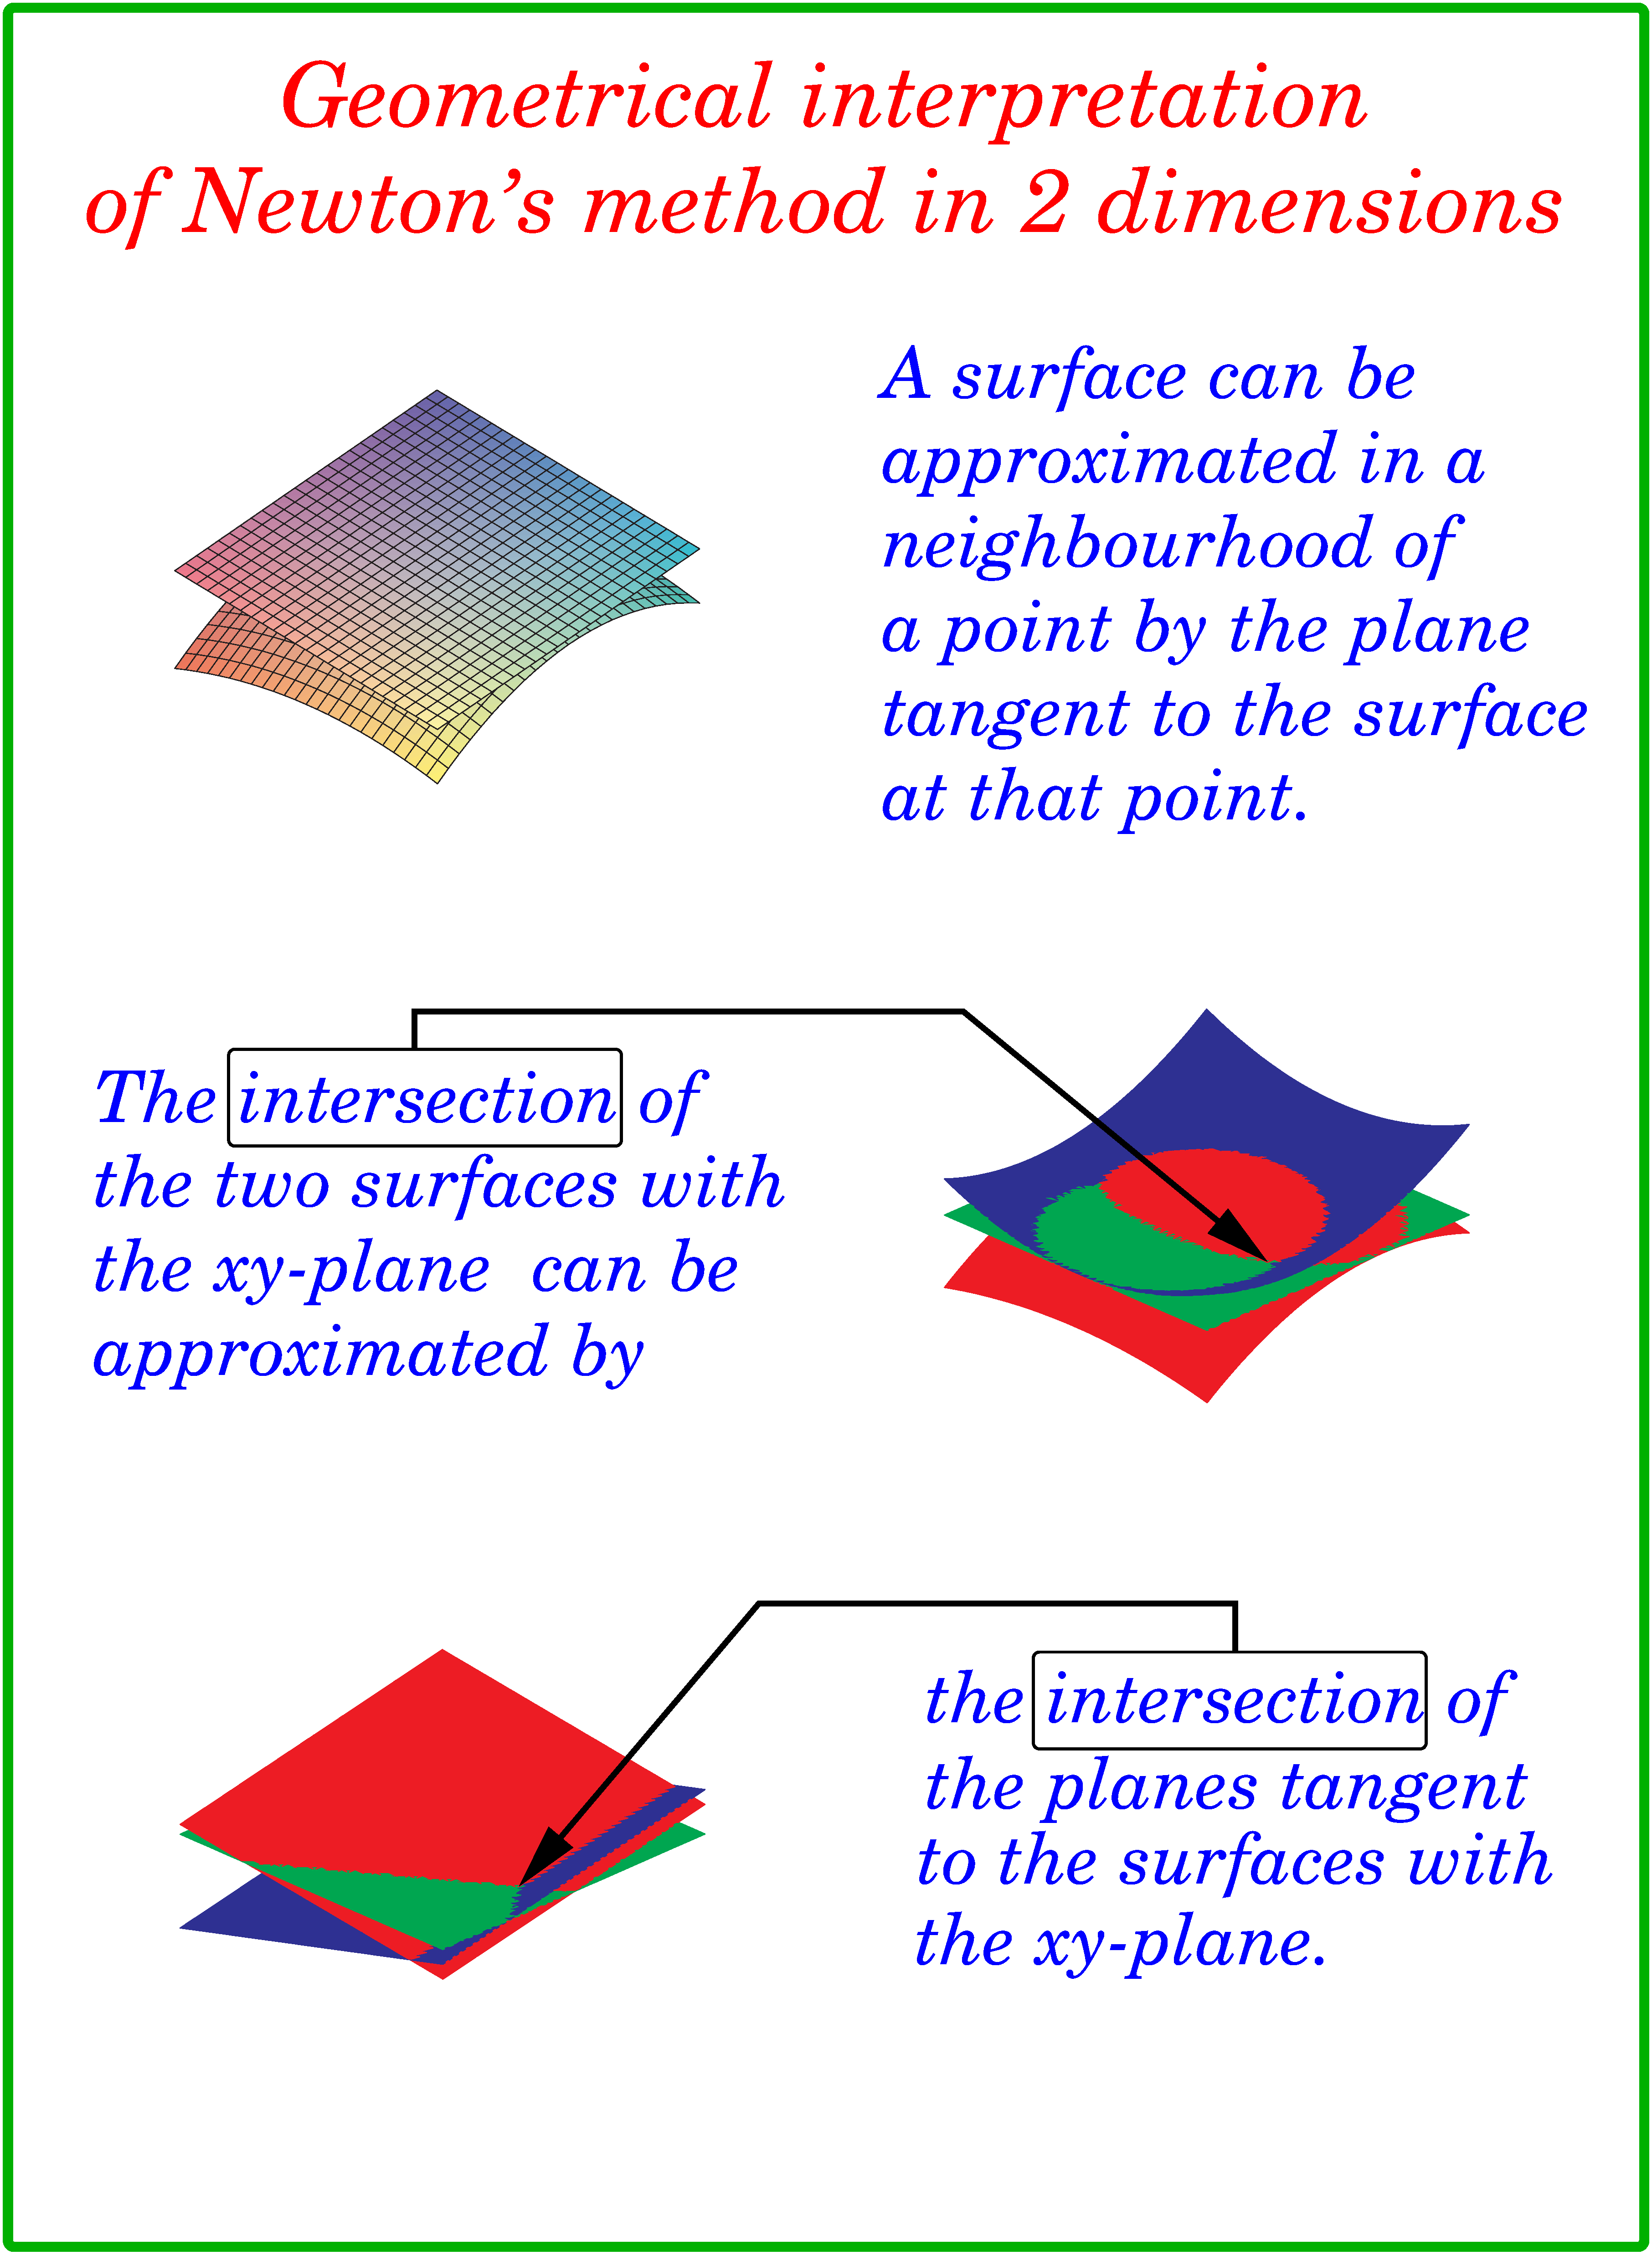
\includegraphics[width=150mm]{figures/Newt2}}
  \caption{\label{fig:Newt2} \it Geometrical meaning of Newton's
    method to solve a system of two nonlinear equations in two
    variables.  The solutions of the system are the intersections of
    the two surfaces with the $xy$-plane.}
\end{figure}

In discussing Newton's method we shall use only $2 \times 2$ systems,
but most of what we say generalises immediately to $n \times n$
systems.   The model problem that we wish to solve is
%
\begin{equation*}
  \begin{cases}
    f_1(x,y) = 0, \\ f_2(x,y) = 0 ,
  \end{cases}
  \quad \Longleftrightarrow \quad
  \bff(\bx) = 0 .
\end{equation*}
%
The easiest way to obtain an expression for Newton's method in two
dimensions is based on the its geometrical interpretation.   We start
by recapping the one dimension case: suppose that we wish to solve the
equation $f(x) = 0$ and that we have evaluated the function at $x_n$.
The next iterate, $x_{n+1}$ is the intersection of the straight line
tangent to the graph of $f(x)$ at $(x_n, f(x_n))$ with the $x$ axis.
The equation of this line is given by the first two terms of the
Taylor expansion of the function $f(x)$ around $x_n$:
%
\begin{equation*}
  y = f(x_n) + f'(x_n) (x - x_n) .
\end{equation*}
%
It intersects the $x$ axis at the point $x_{n+1}$ such that $y=0$, i.e.
%
\begin{equation*}
  0 = f(x_n) + f'(x_n) (x_{n+1} - x_n) \implies
  x_{n+1} =  x_n - \frac{f(x_n)}{f'(x_n)} .
\end{equation*}
%
The geometrical interpretation of Newton's method in two dimensions is
that the iterate $(x_{n+1},y_{n+1})$ is the common point where
the planes tangent to the graph of $f_1(x,y)$ and $f_2(x,y)$ at
$(x_n,y_n)$ intersect the $xy$-plane, i.e.\ the plane $z=0$ (see
Figure~\ref{fig:Newt2}).  The plane tangent to the two surfaces are
%
\begin{align*}
  z &= f_1(x_n,y_n) + (x - x_n) \pdv{f_1}{x}(x_n,y_n) +
  (y - y_n) \pdv{f_1}{y}(x_n,y_n) , \\
  z &= f_2(x_n,y_n) + (x - x_n) \pdv{f_2}{x}(x_n,y_n) +
           (y - y_n) \pdv{f_2}{y}(x_n,y_n) .
\end{align*}
%
At the intersection with the $xy$-plane we have $z=0$.
Therefore the equations for the next iterate are
%
\begin{align}
  f_1(x_n,y_n) + (x_{n+1} - x_n) \pdv{f_1}{x}(x_n,y_n) +
  (y_{n+1} - y_n) \pdv{f_1}{y}(x_n,y_n) &= 0 ,
  \label{eq:f1} \\
  f_2(x_n,y_n) + (x_{n+1} - x_n) \pdv{f_2}{x}(x_n,y_n) +
  (y_{n+1} - y_n) \pdv{f_2}{y}(x_n,y_n) &= 0 .
  \label{eq:f2}
\end{align}
%
We introduce the Jacobian of the function $\bff(\bx)$ at $(x_n,y_n)$,
%
\begin{equation*}
  J(x_n,y_n) =
  \begin{pmatrix}
    \partial_x f_1(x_n,y_n) & \partial_y f_1(x_n,y_n) \\
    \partial_x f_2(x_n,y_n) & \partial_y f_2(x_n,y_n)
  \end{pmatrix}
\end{equation*}
%
and write~(\ref{eq:f1}) and~(\ref{eq:f2}) in matrix notation as
%
\begin{equation*}
  J(x_n,y_n)
  \begin{pmatrix}
    x_{n+1} - x_n \\ y_{n+1} - y_n
  \end{pmatrix}
  =
  \begin{pmatrix}
    - f_1(x_n,y_n) \\ - f_2(x_n,y_n)
  \end{pmatrix}
  ,
\end{equation*}
%
so that the next iterate of Newton's method is
%
\begin{equation}
  \begin{pmatrix}
    x_{n+1} \\ y_{n+1}
  \end{pmatrix}
 =
 \begin{pmatrix}
   x_n \\ y_n
 \end{pmatrix}
 - J^{-1}
 \begin{pmatrix}
   -f_1(x_n,y_n) \\ -f_2(x_n,y_n)
 \end{pmatrix}
 . \label{Newtontwo}
\end{equation}
%
Equation~(\ref{Newtontwo}) generalises to $n$-dimensions as
%
\begin{equation}
  \bx_{n+1} = \bx_{n} -
  \left [ J(\bx_n) \right ]^{-1} \bff(\bx_n) . \label{NewtonRn}
\end{equation}
%
The scheme~(\ref{NewtonRn}) is numerically not convenient, because it
requires the computation of the inverse of the Jacobian.  Therefore,
one normally defines an additional variable
%
\begin{equation*}
  \bz = \bx_{n+1} - \bx_n \implies J \bz = - \bff(\bx_n) ,
\end{equation*}
%
and solves the linear problem for $\bz$ using, for example, Gauss
elimination with pivoting.  Once $\bz$ is known we can obtain
%
\begin{equation*}
  \bx_{n+1} = \bx_n + \bz .
\end{equation*}

\noindent
\textbf{Remark 1} - The initial guess is absolutely crucial and the
method can be very ``touchy''.  However, if we are close enough to the
root and the Jacobian is non singular the convergence is quadratic.

\noindent
\textbf{Remark 2} - Newton's method is very computationally intensive:
it requires the evaluation of $n^2$ derivatives and the solution of an
$n \times n$ linear problem at each iteration.  A multidimensional
version of the secant method has been developed to reduce the number
of computations per step (Broyden algorithm).


\section*{Further reading}

Topics covered here are also covered in
\begin{itemize}
\item Chapter 7 of Linz \& Wang, \textit{Exploring Numerical Methods}
  (QA297 LIN),
\item Chapter 3 of Kincaid \& Cheney, \textit{Numerical Analysis}
  (QA297 KIN),
\item Chapters 1 and 4 of S{\"u}li \& Mayers, \textit{An Introduction
    to Numerical Analysis} (not in library -- includes considerably
  more analysis of the convergence issues).
\end{itemize}
